\documentclass{article}
\usepackage{graphicx} % Required for inserting images
\usepackage[polish]{babel}
\usepackage{hyperref}
\usepackage[T1]{fontenc}
\usepackage{float}
\usepackage{listings}

\title{Dokumentacja - Winda}
\author{Filip Jędrzejewski}
\date{2 Czerwca 2024}

\begin{document}

\maketitle

\section{Opis modelowanego systemu}

Winda to system transportu pionowego, który głównie umożliwia przemieszczanie się osób między różnymi poziomami budynku. Działanie windy opiera się na kilku kluczowych elementach:

\begin{enumerate}
    \item \textbf{Panel przycisków:} Pasażerowie wybierają piętro docelowe, naciskając odpowiedni przycisk na panelu (w windzie lub poza nią - przyciski na poszczególnych piętrach).
    \item \textbf{Sterowanie:} Sygnały z przycisków są przekazywane do sterownika windy, który analizuje żądania i podejmuje decyzje dotyczące ruchu kabiny.
    \item \textbf{Silnik:} Silnik elektryczny porusza kabiną windy w odpowiednim kierunku.
    \item \textbf{Kabina:} Kabina windy porusza się w szybie windowym przewożąc pasażerów.
    \item \textbf{Drzwi:} Drzwi kabiny i drzwi zewnętrzne (piętra) otwierają się i zamykają automatycznie, umożliwiając bezpieczne wejście i wyjście pasażerów.
    \item \textbf{Wyświetlacz:} Wyświetlacz informuje pasażerów o aktualnym położeniu kabiny.
\end{enumerate}

Cykl działania przykładowej windy:

\begin{enumerate}
    \item Pasażer naciska przycisk, wskazując piętro docelowe.
    \item Sterownik windy odbiera sygnał i analizuje go, uwzględniając aktualne położenie kabiny i inne żądania.
    \item Sterownik wysyła polecenie do silnika, aby rozpocząć ruch w odpowiednim kierunku.
    \item Silnik napędza kabinę poruszającą się w szybie windowym.
    \item Gdy kabina osiągnie żądane piętro, sterownik wysyła polecenie do silnika, aby zatrzymać windę.
    \item Sterownik wysyła polecenie do drzwi kabiny i drzwi piętra, aby się otworzyły.
    \item Pasażerowie wchodzą lub wychodzą z windy.
    \item Po określonym czasie lub po naciśnięciu przycisku zamknięcia drzwi, sterownik wysyła polecenie zamknięcia drzwi.
    \item Po zamknięciu drzwi, winda jest gotowa do przyjęcia kolejnego żądania (cykl się powtarza).
\end{enumerate}


\section{Spis komponentów}

\subsection{Komponenty typu \texttt{data}}

\subsubsection{ElevatorState}

Kod:

    \begin{lstlisting}[basicstyle=\ttfamily, keywordstyle=\bfseries]
data ElevatorState
    properties
        Data_Model::Enumerators => ("Idle", "MovingUp", "MovingDown",
                                     "DoorOpening", "DoorClosing");
        Data_Model::Data_Representation => Integer;
        Data_Size => 4 Bytes;
end ElevatorState;

data implementation ElevatorState.impl
end ElevatorState.impl;
    \end{lstlisting}

    \texttt{ElevatorState} to enumerator, który reprezentuje możliwe stany windy. Komponent ten jest używany do śledzenia aktualnego stanu windy w systemie. W podanym modelu zdefiniowano pięć stanów:

    \begin{itemize}
        \item \textbf{Idle:} winda jest bezczynna, nie porusza się i ma zamknięte drzwi.
        \item \textbf{MovingUp:} Winda porusza się w górę.
        \item \textbf{MovingDown:} Winda porusza się w dół.
        \item \textbf{DoorOpening:} Drzwi windy są otwierane.
        \item \textbf{DoorClosing:} Drzwi windy są zamykane.
    \end{itemize}

    \newpage

    \subsubsection{ElevatorAction}

Kod:

    \begin{lstlisting}[basicstyle=\ttfamily, keywordstyle=\bfseries]
data ElevatorAction
end ElevatorAction;

data implementation ElevatorAction.impl
    subcomponents
        targetFloor: data FloorNumber;
        direction: data MotorCommand;
end ElevatorAction.impl;
    \end{lstlisting}

    \texttt{ElevatorAction} jest typem danych służącym do przekazywania informacji o żądanej akcji windy. W implementacji \texttt{ElevatorAction.impl}, widzimy, że składa się z dwóch subkomponentów:

    \begin{itemize}
        \item \textbf{targetFloor:} Określa piętro docelowe, na które winda ma się udać.
        \item \textbf{direction:} Określa kierunek ruchu windy
    \end{itemize}


    \subsubsection{FloorNumber}

    Kod:
    
        \begin{lstlisting}[basicstyle=\ttfamily, keywordstyle=\bfseries]
data FloorNumber
    properties
        Data_Model::Data_Representation => Integer;
        Data_Size => 4 Bytes;
end FloorNumber;

data implementation FloorNumber.impl
end FloorNumber.impl;
        \end{lstlisting}
    
        \texttt{FloorNumber} to typ danych reprezentujący numer piętra w budynku. W kontekście windy, \texttt{FloorNumber} jest używany do określania piętra docelowego, aktualnego piętra windy oraz do wyświetlania informacji o piętrze na panelu sterowania i wyświetlaczu w kabinie.
    

    \subsubsection{ButtonType}

    Kod:
    
    \begin{lstlisting}[basicstyle=\ttfamily, keywordstyle=\bfseries]
data ButtonType
    properties
        Data_Model::Enumerators => ("CallUp", "CallDown", "Cabin");
        Data_Model::Data_Representation => Integer;
        Data_Size => 4 Bytes;
end ButtonType;

data implementation ButtonType.impl
end ButtonType.impl;
    \end{lstlisting}

    \texttt{ButtonType} to enumerator definiujący rodzaje przycisków obecnych w systemie windy. Ten typ danych jest używany w połączeniu z typem \texttt{FloorNumber} w strukturze \texttt{ButtonPress}, aby jednoznacznie określić, który przycisk został naciśnięty i na którym piętrze. Zawiera trzy wartości:

    \begin{itemize}
        \item \textbf{CallUp:} Przycisk wywołania windy na wyższe piętro, umieszczony na zewnątrz kabiny.
        \item \textbf{CallDown:} Przycisk wywołania windy na niższe piętro, umieszczony na zewnątrz kabiny.
        \item \textbf{Floor:} Przycisk wyboru konkretnego piętra, znajdujący się wewnątrz kabiny windy.
    \end{itemize}


    \subsubsection{ButtonPress}

    Kod:
    
    \begin{lstlisting}[basicstyle=\ttfamily, keywordstyle=\bfseries]
data ButtonPress
    properties
        Data_Size => 8 Bytes; 
end ButtonPress;

data implementation ButtonPress.impl
    subcomponents
        floor: data FloorNumber;
        button_type: data ButtonType;
end ButtonPress.impl;
    \end{lstlisting}

    \texttt{ButtonPress} to struktura reprezentująca zdarzenie naciśnięcia przycisku w windzie. Zawiera ona dwa elementy:

    \begin{itemize}
        \item \textbf{floor:} Przechowuje numer piętra, na którym przycisk został naciśnięty (lub na jakie ma się udać).
        \item \textbf{button\_type:} Określa rodzaj naciśniętego przycisku (góra, dół lub piętro).
    \end{itemize}

    Te informacje są kluczowe dla systemu sterowania windą, ponieważ umożliwiają mu określenie, na które piętro winda powinna się udać i w jakim kierunku.


    \newpage
    
    \subsubsection{MotorCommand}

    Kod:
    
    \begin{lstlisting}[basicstyle=\ttfamily, keywordstyle=\bfseries]
data MotorCommand
    properties
        Data_Model::Enumerators => ("Up", "Down", "Stop");
        Data_Model::Data_Representation => Integer;
        Data_Size => 4 Bytes;
end MotorCommand;

data implementation MotorCommand.impl
end MotorCommand.impl;
    \end{lstlisting}

    \texttt{MotorCommand} to enumerator definiujący możliwe polecenia sterujące dla silnika windy. Kontroler silnika interpretuje to polecenie i steruje silnikiem windy zgodnie z nim. Zawiera trzy wartości:

    \begin{itemize}
        \item \textbf{Up:} Polecenie ruchu windy w górę.
        \item \textbf{Down:} Polecenie ruchu windy w dół.
        \item \textbf{Stop:} Polecenie zatrzymania windy
    \end{itemize}


    \subsubsection{DoorCommand}

    Kod:
    
    \begin{lstlisting}[basicstyle=\ttfamily, keywordstyle=\bfseries]
data DoorCommand
    properties
        Data_Model::Enumerators => ("Open", "Close");
        Data_Model::Data_Representation => Integer;
        Data_Size => 4 Bytes;
end DoorCommand;

data implementation DoorCommand.impl
end DoorCommand.impl;
    \end{lstlisting}

    \texttt{DoorCommand} to enumerator określający możliwe polecenia dla drzwi windy. Zawiera dwie wartości:

    \begin{itemize}
        \item \textbf{Open:} Polecenie otwarcia drzwi windy.
        \item \textbf{Close:} Polecenie zamknięcia drzwi windy.
    \end{itemize}

    \newpage

    \subsubsection{DoorState}

    Kod:
    
    \begin{lstlisting}[basicstyle=\ttfamily, keywordstyle=\bfseries]
data DoorState
    properties
        Data_Model::Enumerators => ("Opened", "Closed", "Opening", "Closing");
        Data_Model::Data_Representation => Integer;
        Data_Size => 4 Bytes;
end DoorState;

data implementation DoorState.impl
end DoorState.impl;
    \end{lstlisting}

    \texttt{DoorState} to enumerator reprezentujący możliwe stany drzwi windy. Zawiera on cztery wartości:

    \begin{itemize}
        \item \textbf{Opened:} Drzwi są całkowicie otwarte.
        \item \textbf{Closed:} Drzwi są całkowicie zamknięte.
        \item \textbf{Opening:} Drzwi są w trakcie otwierania.
        \item \textbf{Closing:} Drzwi są w trakcie zamykania.
    \end{itemize}



    \subsection{Komponenty typu \texttt{thread}}

    
    \subsubsection{ButtonPanelThread}

    Kod:
    
    \begin{lstlisting}[basicstyle=\ttfamily, keywordstyle=\bfseries]
thread ButtonPanelThread
    features
        button_press_in: in event data port ButtonPress;
        button_data_out: out data port ButtonPress;
    properties
        SEI::MIPSBudget => 0.8 mips;
end ButtonPanelThread;

thread implementation ButtonPanelThread.impl
end ButtonPanelThread.impl;
    \end{lstlisting}

    \texttt{ButtonPanelThread} jest wątkiem odpowiedzialnym za obsługę panelu przycisków w windzie. Jego głównym zadaniem jest odczytywanie sygnałów z przycisków i przekazywanie informacji o naciśnięciach do \texttt{ButtonPanelController}. Wątek \texttt{ButtonPanelThread} jest kluczowym elementem systemu windy, ponieważ umożliwia pasażerom komunikowanie swoich żądań do systemu.

    
    \subsubsection{ElevatorLogicThread}

    Kod:
    
    \begin{lstlisting}[basicstyle=\ttfamily, keywordstyle=\bfseries]
thread ElevatorLogicThread
    features
        button_data_in: in data port ButtonPress;
        action_data_out: out data port ElevatorAction;
    properties
        SEI::MIPSBudget => 0.8 mips;
end ElevatorLogicThread;

thread implementation ElevatorLogicThread.impl
end ElevatorLogicThread.impl;
    \end{lstlisting}

    \texttt{ElevatorLogicThread} jest wątkiem odpowiedzialnym za podejmowanie podstawowych decyzji dotyczących działania windy. Jego głównym zadaniem jest analiza żądań pasażerów (\texttt{ButtonPress}) i generowanie akcji (\texttt{ElevatorAction}) w odpowiedzi na te żądania. Wątek ten bierze pod uwagę aktualny stan windy (np. piętro, kierunek ruchu) oraz informacje o naciśniętych przyciskach, aby zdecydować, na które piętro winda powinna się udać.



    \subsubsection{ElevatorLogicTransformThread}

    Kod:
    
    \begin{lstlisting}[basicstyle=\ttfamily, keywordstyle=\bfseries]
thread ElevatorLogicTransformThread
    features
        action_data_in: in data port ElevatorAction;
        motor_state_in: in data port ElevatorState;
        motor_state_out: out data port MotorCommand;
        floor_data_out: out data port FloorNumber;
        door_command_out: out data port DoorCommand;
    properties
        SEI::MIPSBudget => 0.8 mips;
end ElevatorLogicTransformThread;

thread implementation ElevatorLogicTransformThread.impl
end ElevatorLogicTransformThread.impl;
    \end{lstlisting}

    \texttt{ElevatorLogicTransformThread} jest wątkiem odpowiedzialnym za przekształcanie akcji windy (\texttt{ElevatorAction}) na konkretne polecenia sterujące dla silnika (\texttt{MotorCommand}) i drzwi (\texttt{DoorCommand}). Dodatkowo, wątek ten wysyła informację do kontrolera wyświetlacza (\texttt{DisplayController}).


    \newpage

    \subsubsection{MotorControlThread}

    Kod:
    
    \begin{lstlisting}[basicstyle=\ttfamily, keywordstyle=\bfseries]
thread MotorControlThread
    features
        motor_state_in: in data port MotorCommand;
        motor_state_out: out data port ElevatorState;
        motor_command_out: out data port MotorCommand;
    properties
        SEI::MIPSBudget => 0.8 mips;
end MotorControlThread;

thread implementation MotorControlThread.impl
end MotorControlThread.impl;
    \end{lstlisting}

    \texttt{MotorControlThread} jest wątkiem odpowiedzialnym za bezpośrednie sterowanie silnikiem windy. Odbiera on polecenia od \texttt{MotorController}, które określają, czy silnik ma się poruszać w górę, w dół, czy też zatrzymać. Na podstawie tych poleceń, wątek generuje odpowiednie sygnały sterujące dla silnika i monitoruje jego stan.


    \subsubsection{DisplayThread}

    Kod:
    
    \begin{lstlisting}[basicstyle=\ttfamily, keywordstyle=\bfseries]
thread DisplayThread
    features
        floor_data_in: in data port FloorNumber;
        display_output: out data port FloorNumber;
    properties
        SEI::MIPSBudget => 0.8 mips; 
end DisplayThread;

thread implementation DisplayThread.impl
end DisplayThread.impl;
    \end{lstlisting}

    \texttt{DisplayThread} jest wątkiem odpowiedzialnym za aktualizację wyświetlacza windy. Odbiera on informację o aktualnym piętrze od \texttt{DisplayController} i wyświetla ją na panelu w kabinie windy. Wątek ten działa w sposób ciągły, aktualizując wyświetlacz za każdym razem, gdy winda zmienia piętro. Jego zadaniem jest informowanie, za pomocą wyświetlacza (\texttt{Display}), pasażerów o aktualnym położeniu windy.


    \newpage

    \subsubsection{CabinControlThread}

    Kod:
    
    \begin{lstlisting}[basicstyle=\ttfamily, keywordstyle=\bfseries]
thread CabinControlThread
    features
        door_command_in: in data port DoorCommand;
        door_state_in: in data port DoorState;
        door_open: out event port;
        door_close: out event port;
    properties
        SEI::MIPSBudget => 0.8 mips;
end CabinControlThread;

thread implementation CabinControlThread.impl
end CabinControlThread.impl;
    \end{lstlisting}

    \texttt{CabinControlThread} jest wątkiem odpowiedzialnym za sterowanie drzwiami kabiny windy. Odbiera on polecenia od \texttt{CabinController}, które określają, czy drzwi mają być otwarte czy zamknięte. Wątek ten generuje odpowiednie sygnały sterujące dla mechanizmu drzwi. Działanie tego wątku jest kluczowe dla bezpieczeństwa i wygody pasażerów, zapewniając prawidłowe funkcjonowanie drzwi windy.






    \subsection{Komponenty typu \texttt{process}}

    
    \subsubsection{ButtonPanelController}

    Kod:
    
    \begin{lstlisting}[basicstyle=\ttfamily, keywordstyle=\bfseries]
process ButtonPanelController
    features
        receive_button_press: in data port ButtonPress;
        send_button_data: out data port ButtonPress;
end ButtonPanelController;

process implementation ButtonPanelController.impl
    subcomponents
        buttonPanelThread: thread ButtonPanelThread.impl;
    connections
        c1: port receive_button_press -> buttonPanelThread.button_press_in;
        c2: port buttonPanelThread.button_data_out -> send_button_data;
end ButtonPanelController.impl;
    \end{lstlisting}

    \texttt{ButtonPanelController} jest procesem odpowiedzialnym za zarządzanie panelem przycisków w windzie. Jego głównym zadaniem jest odbiór informacji o naciśniętych przyciskach z panelu i przekazanie tych danych do kontrolera logiki windy (\texttt{ElevatorLogicController}). Ten proces umożliwia pasażerom wybór piętra docelowego.





    \subsubsection{ElevatorLogicController}

    Kod:
    
    \begin{lstlisting}[basicstyle=\ttfamily, keywordstyle=\bfseries]
process ElevatorLogicController
    features
        receive_button_data: in data port ButtonPress;
        receive_motor_state_data: in data port ElevatorState;
        send_floor_data: out data port FloorNumber;
        send_door_command: out data port DoorCommand;
        send_action: out data port MotorCommand;
end ElevatorLogicController;

process implementation ElevatorLogicController.impl
    subcomponents
        logicThread: thread ElevatorLogicThread.impl;
        transformThread: thread ElevatorLogicTransformThread.impl;
    connections
        c1: port receive_button_data -> logicThread.button_data_in;
        c2: port receive_motor_state_data -> transformThread.motor_state_in;
        c3: port logicThread.action_data_out -> transformThread.action_data_in;
        c5: port transformThread.floor_data_out -> send_floor_data;
        c6: port transformThread.door_command_out -> send_door_command;
        c7: port transformThread.motor_state_out -> send_action; 
end ElevatorLogicController.impl;
    \end{lstlisting}

    \texttt{ElevatorLogicController}  jest centralnym procesem odpowiedzialnym za logikę sterowania windą. Odbiera on informacje o naciśniętych przyciskach oraz aktualny stan windy. Na podstawie tych danych, podejmuje decyzje dotyczące kierunku ruchu windy, piętra docelowego oraz stanu drzwi, wysyłając odpowiednie polecenia do kolejnych komponentów.



    \newpage

    \subsubsection{DisplayController}

    Kod:
    
    \begin{lstlisting}[basicstyle=\ttfamily, keywordstyle=\bfseries]
process DisplayController
    features
        receive_floor_data: in data port FloorNumber;
        display_output: out data port FloorNumber;
end DisplayController;

process implementation DisplayController.impl
    subcomponents
        displayThread: thread DisplayThread.impl;
    connections
        c1: port receive_floor_data -> displayThread.floor_data_in;
        c2: port displayThread.display_output -> display_output;
end DisplayController.impl;
    \end{lstlisting}

    \texttt{DisplayController} jest procesem odpowiedzialnym za zarządzanie wyświetlaczem windy. Jego głównym zadaniem jest odbieranie informacji o aktualnym piętrze od \texttt{ElevatorLogicController} i przekazywanie ich do wątku \texttt{DisplayThread}, który zajmuje się fizyczną aktualizacją wyświetlacza.





    \subsubsection{CabinController}

    Kod:
    
    \begin{lstlisting}[basicstyle=\ttfamily, keywordstyle=\bfseries]
process CabinController
    features
        receive_door_command: in data port DoorCommand;
        receive_door_state: in data port DoorState;
        door_open: out event port;
        door_close: out event port;
end CabinController;

process implementation CabinController.impl
    subcomponents
        cabinThread: thread CabinControlThread.impl;
    connections
        c1: port receive_door_command -> cabinThread.door_command_in;
        c2: port receive_door_state -> cabinThread.door_state_in;
        c3: port cabinThread.door_open -> door_open;
        c4: port cabinThread.door_close -> door_close;
end CabinController.impl;
    \end{lstlisting}

    \texttt{CabinController} jest procesem odpowiedzialnym za zarządzanie drzwiami kabiny windy. Zapewnia, że drzwi otwierają się i zamykają tylko w odpowiednich momentach, na przykład gdy winda jest zatrzymana na piętrze, oraz że drzwi są bezpiecznie zamknięte podczas jazdy windy.



    \subsubsection{MotorController}

    Kod:
    
    \begin{lstlisting}[basicstyle=\ttfamily, keywordstyle=\bfseries]
process MotorController
    features
        receive_motor_command: in data port MotorCommand;
        send_motor_state: out data port ElevatorState;
end MotorController;

process implementation MotorController.impl
    subcomponents
        motorThread: thread MotorControlThread.impl; 
    connections
        c1: port receive_motor_command -> motorThread.motor_state_in;
        c2: port motorThread.motor_state_out -> send_motor_state;
end MotorController.impl;
    \end{lstlisting}

    \texttt{MotorController} jest procesem pełniącym rolę pośrednika między logiką sterowania windą, a silnikiem. Jego głównym zadaniem jest odbieranie poleceń ruchu i przekazywanie ich do wątku \texttt{MotorControlThread}, który bezpośrednio steruje silnikiem.










    \subsection{Komponenty typu \texttt{bus}}

    
    \subsubsection{CANBus}

    Kod:
    
    \begin{lstlisting}[basicstyle=\ttfamily, keywordstyle=\bfseries]
bus CANBus
    properties
        SEI::GrossWeight => 0.075kg;
        SEI::BandWidthCapacity => 1.0 Mbps; 
end CANBus;

bus implementation CANBus.impl
end CANBus.impl;
    \end{lstlisting}

    \texttt{CANBus} jest magistralą komunikacyjną typu CAN (Controller Area Network). Służy ona do wymiany danych między różnymi komponentami systemu windy. Magistrala CAN zapewnia niezawodną i szybką komunikację w czasie rzeczywistym, co jest kluczowe dla prawidłowego działania systemu windy.


    \newpage

    \subsubsection{HWConnection}

    Kod:
    
    \begin{lstlisting}[basicstyle=\ttfamily, keywordstyle=\bfseries]
bus HWConnection
    properties
        SEI::GrossWeight => 0.075kg;
        SEI::BandWidthCapacity => 1000.0 Mbps;
end HWConnection;

bus implementation HWConnection.impl
end HWConnection.impl;
    \end{lstlisting}

    \texttt{HWConnection} reprezentuje magistralę sprzętową, która umożliwia szybką komunikację między procesorem (\texttt{CPU}) a pamięcią RAM (\texttt{RAM}). Jest to wewnętrzne połączenie o wysokiej przepustowości, które służy do przesyłania informacji między tymi dwoma komponentami systemu.










    \subsection{Komponenty typu \texttt{memory}}

    
    \subsubsection{RAM}

    Kod:
    
    \begin{lstlisting}[basicstyle=\ttfamily, keywordstyle=\bfseries]
memory RAM
    features
        hwcAccess: requires bus access HWConnection;
    properties
        SEI::GrossWeight => 0.025kg;
end RAM;

memory implementation RAM.impl
end RAM.impl;
    \end{lstlisting}

    \texttt{RAM} to komponent reprezentujący pamięć operacyjną systemu windy. Jest to miejsce, w którym przechowywane są dane tymczasowe, instrukcje programu oraz zmienne wykorzystywane przez procesor (\texttt{CPU}) podczas działania windy. 



    \newpage

    \subsection{Komponenty typu \texttt{processor}}

    
    \subsubsection{CPU}

    Kod:
    
    \begin{lstlisting}[basicstyle=\ttfamily, keywordstyle=\bfseries]
processor CPU
    features
        canBusAccess: requires bus access CANBus;
        hwcAccess: requires bus access HWConnection;
    properties
        Scheduling_Protocol => (Round_Robin_Protocol);
        Clock_Period => 1 ms;	
        Timing_Properties::Processor_Capacity => 1.0 MIPS;
        SEI::MIPSCapacity => 1.2 mips;
        SEI::GrossWeight => 0.05kg;
end CPU;

processor implementation CPU.impl
end CPU.impl;
    \end{lstlisting}

    \texttt{CPU} to centralny element obliczeniowy systemu windy, odpowiedzialny za wykonywanie instrukcji oprogramowania sterującego windą. Jest to kluczowy komponent, który przetwarza dane wejściowe z różnych czujników i przycisków, podejmuje decyzje dotyczące ruchu windy (kierunek, prędkość, zatrzymanie) oraz steruje innymi urządzeniami, takimi jak: silnik, drzwi i wyświetlacz. 




    \subsection{Komponenty typu \texttt{device}}

    
    \subsubsection{ButtonPanel}

    Kod:
    
    \begin{lstlisting}[basicstyle=\ttfamily, keywordstyle=\bfseries]
device ButtonPanel
    features
        button_press: out data port ButtonPress;
        bus_access: requires bus access CANBus;
    properties
        SEI::GrossWeight => 1.0kg;
end ButtonPanel;

device implementation ButtonPanel.impl
end ButtonPanel.impl;
    \end{lstlisting}

    \texttt{ButtonPanel} jest urządzeniem, które reprezentuje panel przycisków wewnątrz i na zewnątrz windy. Zadaniem tego panelu jest umożliwienie pasażerom wydawanie poleceń windzie, takich jak wybór piętra docelowego czy wezwanie windy na dane piętro.


    \newpage

    \subsubsection{Cabin}

    Kod:
    
    \begin{lstlisting}[basicstyle=\ttfamily, keywordstyle=\bfseries]
device Cabin
    features
        door_state: out data port DoorState;
        door_open: in event port;
        door_close: in event port;
    properties
        SEI::GrossWeight => 150.0kg;
end Cabin;

device implementation Cabin.impl
end Cabin.impl;
    \end{lstlisting}

    \texttt{Cabin} reprezentuje kabinę windy, czyli przestrzeń, w której przebywają pasażerowie podczas jazdy. 




    \subsubsection{Motor}

    Kod:
    
    \begin{lstlisting}[basicstyle=\ttfamily, keywordstyle=\bfseries]
device Motor
    features
        motor_state_in: in data port ElevatorState;
        motor_state_out: out data port ElevatorState;
    properties
        SEI::GrossWeight => 5.0kg;
end Motor;

device implementation Motor.impl
end Motor.impl;
    \end{lstlisting}

    \texttt{Motor} to urządzenie, które reprezentuje silnik elektryczny napędzający windę. Silnik ten jest odpowiedzialny za ruch kabiny w górę i w dół szybu windowego.



    \subsubsection{Display}

    Kod:
    
    \begin{lstlisting}[basicstyle=\ttfamily, keywordstyle=\bfseries]
device Display
    features
        display_input: in data port FloorNumber; 
end Display;

device implementation Display.impl
end Display.impl;
    \end{lstlisting}

    \texttt{Display} jest urządzeniem odpowiedzialnym za prezentowanie informacji pasażerom windy. Jego głównym zadaniem jest wyświetlanie aktualnego piętra, na którym znajduje się kabina. 


    \subsubsection{ElevatorController}

    Kod:
    
    \begin{lstlisting}[basicstyle=\ttfamily, keywordstyle=\bfseries]
device ElevatorController
    features
        action_receive: in data port MotorCommand;
        motor_command: out data port MotorCommand;
        motor_state_receive: in data port ElevatorState;
        motor_state_send: out data port ElevatorState;
        bus_access: requires bus access CANBus;
    properties
        SEI::GrossWeight => 0.5kg;
        Period => 100ms;
        Dispatch_Protocol => Periodic;
end ElevatorController;

device implementation ElevatorController.impl
end ElevatorController.impl;
    \end{lstlisting}

    \texttt{ElevatorController}  to urządzenie pełniące rolę głównego sterownika sprzętowego windy. Ten komponent jest kluczowy dla prawidłowego działania windy, ponieważ integruje logikę sterowania z fizycznymi elementami windy, takimi jak silnik i drzwi.




    \subsection{Komponenty typu \texttt{system}}

    
    \subsubsection{ElevatorSystem}

    Kod:
    
    \begin{lstlisting}[basicstyle=\ttfamily, keywordstyle=\bfseries]
system implementation ElevatorSystem.impl
    subcomponents
        button_panel: device ButtonPanel.impl;
        cabin: device Cabin.impl;
        motor: device Motor.impl;
        elevatorController: device ElevatorController.impl;
        display: device Display.impl;

        cpu: processor CPU.impl;
        ram: memory RAM.impl;
        can_bus: bus CANBus.impl;
        hwc: bus HWConnection.impl;

        buttonPanelController: process ButtonPanelController.impl;
        elevatorLogicController: process ElevatorLogicController.impl;
        displayController: process DisplayController.impl;
        cabinController: process CabinController.impl;
        motorController: process MotorController.impl;
    
    

    connections
        -- ButtonPanel connections
        c1: bus access button_panel.bus_access -> can_bus;
        c2: port button_panel.button_press -> buttonPanelController.receive_button_press;
    
        -- ElevatorController connections
        c3: bus access elevatorController.bus_access -> can_bus;
        c4: port elevatorController.motor_command -> motorController.receive_motor_command;
        c5: port motorController.send_motor_state -> motor.motor_state_in;
        c6: port motor.motor_state_out -> elevatorController.motor_state_receive;
        c7: port elevatorController.motor_state_send -> elevatorLogicController.receive_motor_state_data;
        c8: port elevatorLogicController.send_action -> elevatorController.action_receive;  
    
        -- CPU connections
        c9: bus access cpu.hwcAccess -> hwc;
        c10: bus access cpu.canBusAccess -> can_bus;
    
        -- RAM connection
        c11: bus access ram.hwcAccess -> hwc;
    
        -- Process connections
        c12: port buttonPanelController.send_button_data -> elevatorLogicController.receive_button_data;
        c13: port elevatorLogicController.send_floor_data -> displayController.receive_floor_data;
        c14: port elevatorLogicController.send_door_command -> cabinController.receive_door_command;
        c15: port cabin.door_state -> cabinController.receive_door_state;
    
        -- Cabin connections
        c16: port cabinController.door_open -> cabin.door_open;
        c17: port cabinController.door_close -> cabin.door_close;
    
        -- Display connection
        c18: port displayController.display_output -> display.display_input;
        
    properties
        -- Bindings
        Actual_Processor_Binding => (reference(cpu)) applies to buttonPanelController;
        Actual_Processor_Binding => (reference(cpu)) applies to elevatorLogicController;
        Actual_Processor_Binding => (reference(cpu)) applies to displayController;
        Actual_Processor_Binding => (reference(cpu)) applies to cabinController;
        Actual_Processor_Binding => (reference(cpu)) applies to motorController;

        --Other
    	SEI::MIPSCapacity => 2.4 mips;
        
end ElevatorSystem.impl;
    \end{lstlisting}

    \texttt{ElevatorSystem} reprezentuje cały system windy jako całość. Jest to komponent typu system, który integruje wszystkie elementy składowe windy. Model \texttt{ElevatorSystem} definiuje hierarchiczną strukturę systemu windy, określając zależności i połączenia między poszczególnymi komponentami, co umożliwia analizę i weryfikację poprawności działania całego systemu.



\section{Schemat systemu}


\begin{figure}[H]
    \centering
    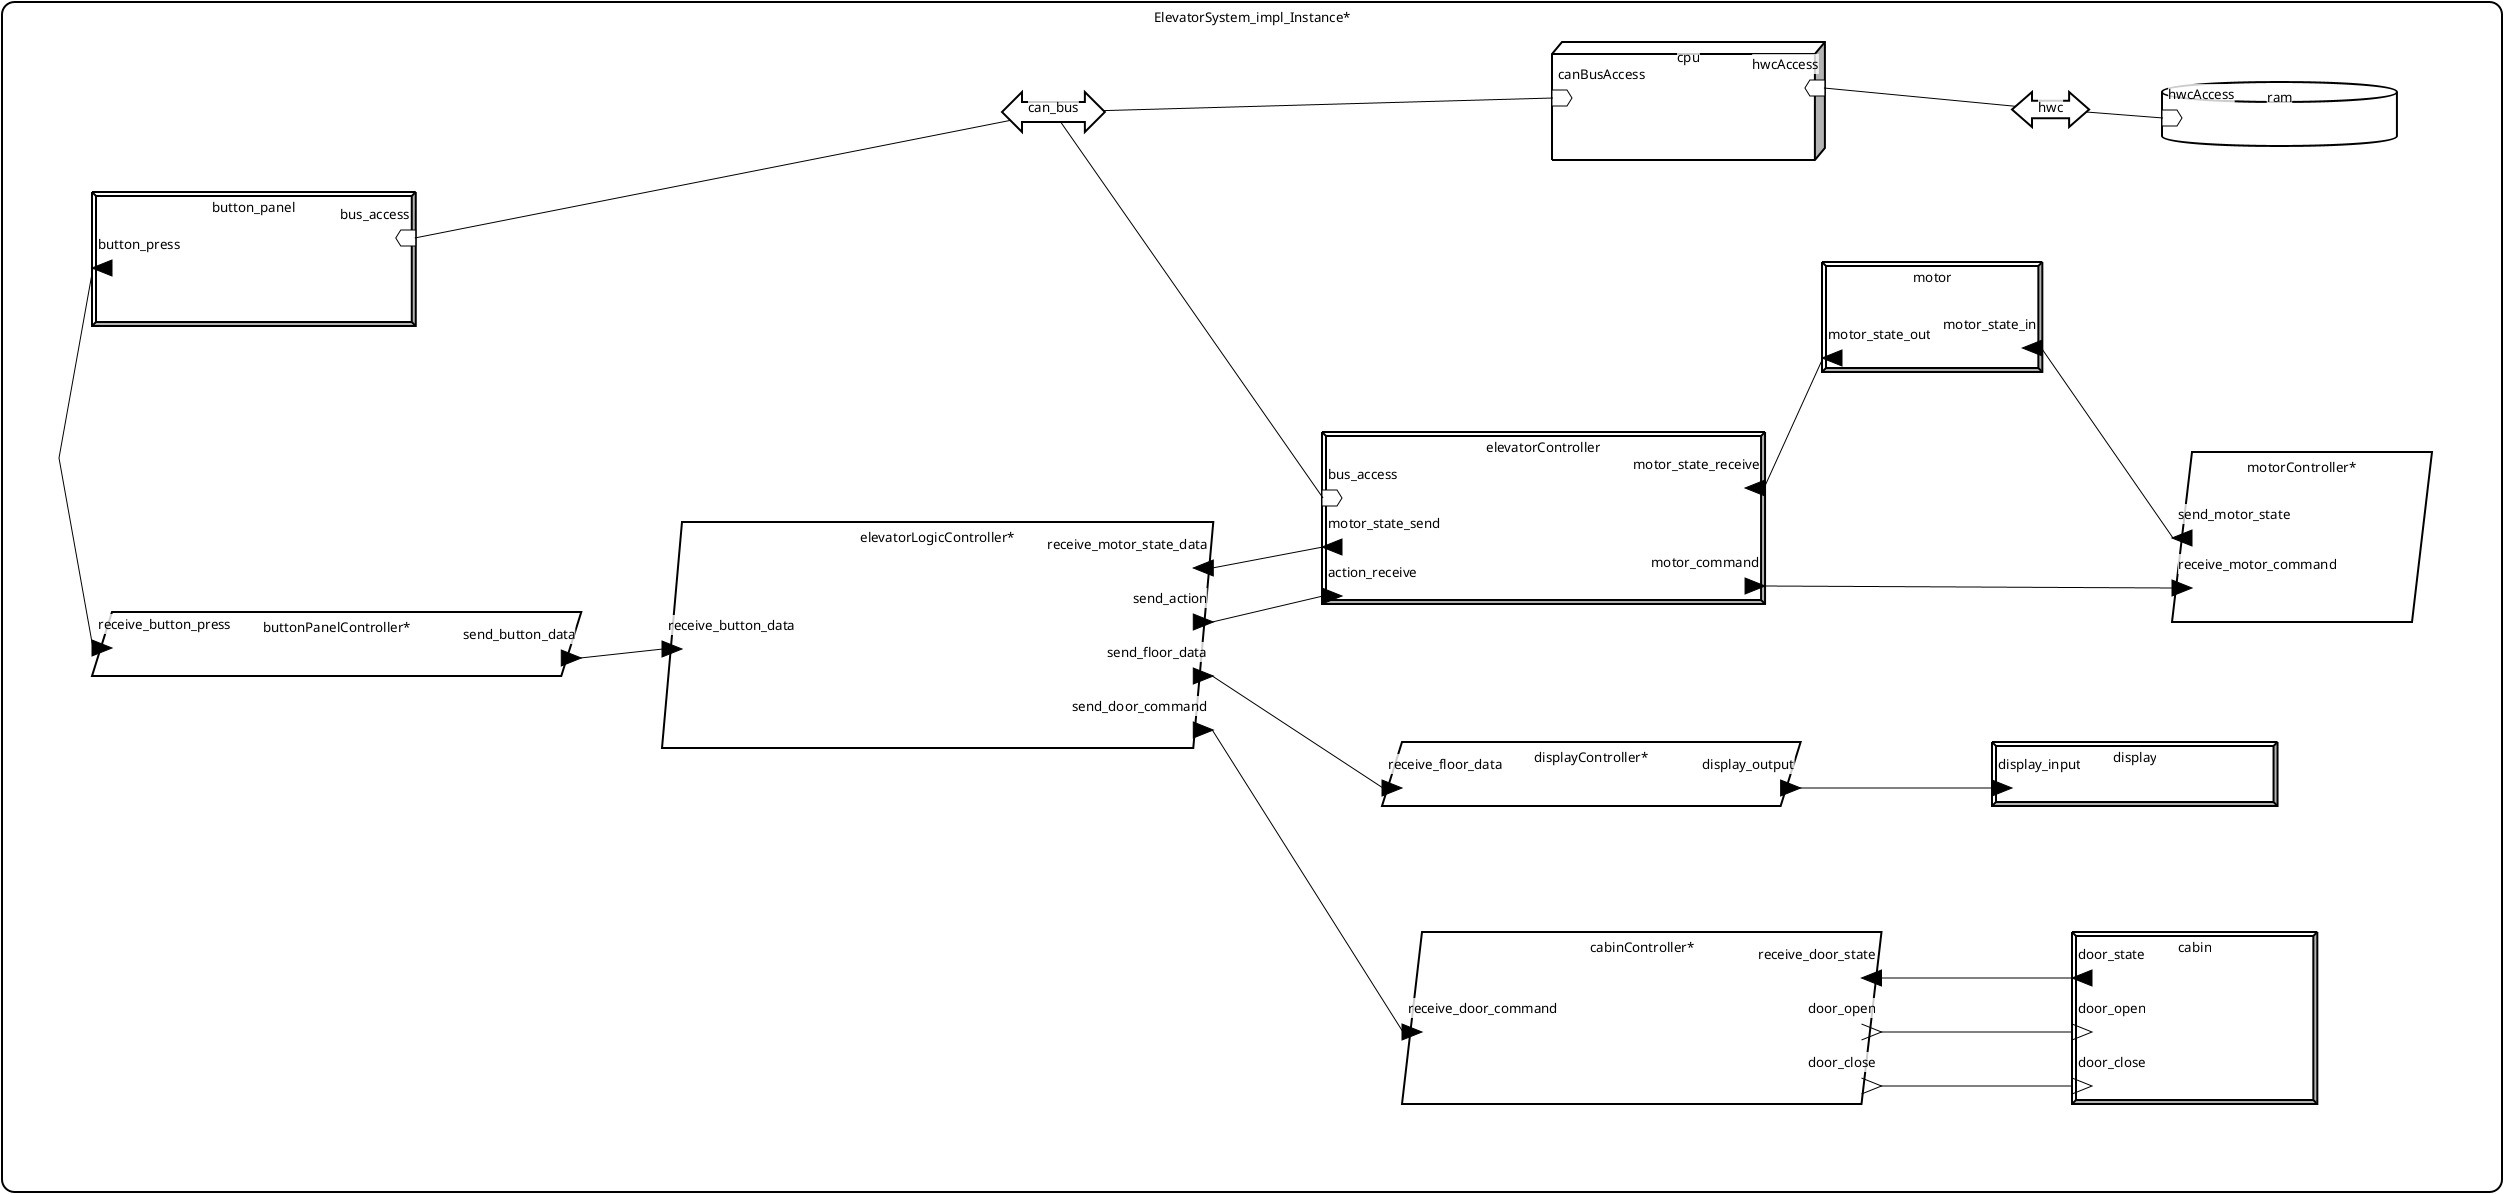
\includegraphics[width=1.2\linewidth]{./images/schema.png}
\end{figure}

\section{Analiza systemu}

\subsection{Statystyki systemu}


\begin{center}
    \begin{tabular}{|c|c|}
        \hline
        \textbf{Elementy modelu} & \textbf{Liczba} \\
        \hline
        Komponenty ogółem & 21 \\
        Komponenty \texttt{bus} & 2 \\
        Komponenty \texttt{device} & 5 \\
        Komponenty \texttt{memory} & 1 \\
        Komponenty \texttt{process} & 5 \\
        Komponenty \texttt{processor} & 1 \\
        Komponenty \texttt{system} & 1 \\
        Komponenty \texttt{thread} & 6 \\
        Połączenia & 19 \\
        \hline
    \end{tabular}
\end{center}

\subsection{Całkowita masa systemu}

Wyniki analizy \textit{Sum of weights}:
\newline

\texttt{[L] Sum of weights / gross weight is 156.975 kg (no limit specified).}











\end{document}